\documentclass[14pt]{extbook}
\usepackage{multicol, enumerate, enumitem, hyperref, color, soul, setspace, parskip, fancyhdr} %General Packages
\usepackage{amssymb, amsthm, amsmath, bbm, latexsym, units, mathtools} %Math Packages
\everymath{\displaystyle} %All math in Display Style
% Packages with additional options
\usepackage[headsep=0.5cm,headheight=12pt, left=1 in,right= 1 in,top= 1 in,bottom= 1 in]{geometry}
\usepackage[usenames,dvipsnames]{xcolor}
\usepackage{dashrule}  % Package to use the command below to create lines between items
\newcommand{\litem}[1]{\item#1\hspace*{-1cm}\rule{\textwidth}{0.4pt}}
\pagestyle{fancy}
\lhead{Progress Quiz 9}
\chead{}
\rhead{Version C}
\lfoot{8590-6105}
\cfoot{}
\rfoot{Fall 2020}
\begin{document}

\begin{enumerate}
\litem{
Describe the end behavior of the polynomial below.\[ f(x) = -6(x + 4)^{5}(x - 4)^{10}(x + 8)^{2}(x - 8)^{2} \]\begin{enumerate}[label=\Alph*.]
\begin{multicols}{2}\item 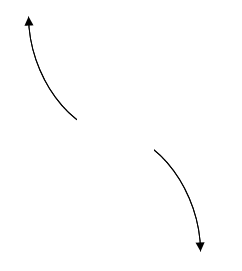
\includegraphics[width = 0.3\textwidth]{../Figures/polyEndBehaviorAC.png}\item 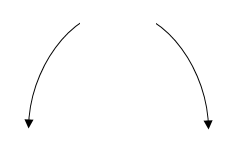
\includegraphics[width = 0.3\textwidth]{../Figures/polyEndBehaviorBC.png}\item 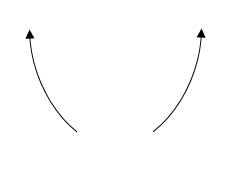
\includegraphics[width = 0.3\textwidth]{../Figures/polyEndBehaviorCC.png}\item 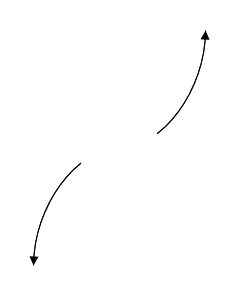
\includegraphics[width = 0.3\textwidth]{../Figures/polyEndBehaviorDC.png}\end{multicols}\item None of the above.
\end{enumerate} }
\litem{
Which of the following equations \textit{could} be of the graph presented below?
\begin{center}
    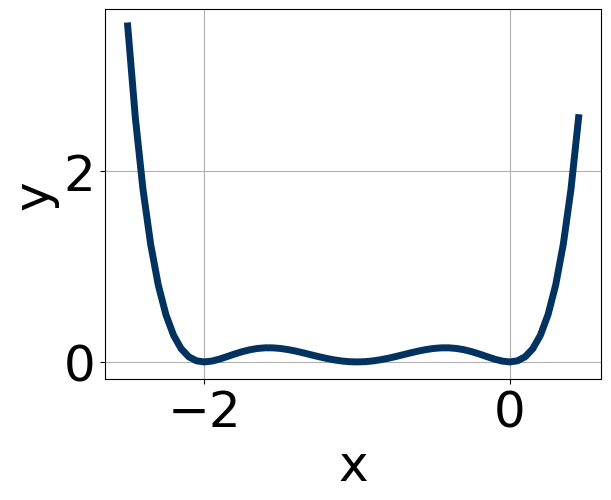
\includegraphics[width=0.5\textwidth]{../Figures/polyGraphToFunctionCopyC.png}
\end{center}
\begin{enumerate}[label=\Alph*.]
\item \( -3x^{4} (x + 1)^{8} (x + 2)^{7} \)
\item \( 3x^{10} (x + 1)^{9} (x + 2)^{9} \)
\item \( -10x^{6} (x + 1)^{6} (x + 2)^{8} \)
\item \( 14x^{8} (x + 1)^{10} (x + 2)^{5} \)
\item \( 18x^{8} (x + 1)^{8} (x + 2)^{8} \)

\end{enumerate} }
\litem{
Construct the lowest-degree polynomial given the zeros below. Then, choose the intervals that contain the coefficients of the polynomial in the form $ax^3+bx^2+cx+d$.\[ \frac{1}{4}, \frac{-1}{5}, \text{ and } \frac{1}{2} \]\begin{enumerate}[label=\Alph*.]
\item \( a \in [38, 42], b \in [-22.1, -20.7], c \in [-1.03, 0.65], \text{ and } d \in [0.99, 2.17] \)
\item \( a \in [38, 42], b \in [-6.3, -1.7], c \in [-8.44, -6.66], \text{ and } d \in [-2.34, -0.38] \)
\item \( a \in [38, 42], b \in [-18.8, -14.4], c \in [-4.18, -1.92], \text{ and } d \in [0.99, 2.17] \)
\item \( a \in [38, 42], b \in [19.4, 22.1], c \in [-1.03, 0.65], \text{ and } d \in [-2.34, -0.38] \)
\item \( a \in [38, 42], b \in [-22.1, -20.7], c \in [-1.03, 0.65], \text{ and } d \in [-2.34, -0.38] \)

\end{enumerate} }
\litem{
Construct the lowest-degree polynomial given the zeros below. Then, choose the intervals that contain the coefficients of the polynomial in the form $ax^3+bx^2+cx+d$.\[ \frac{1}{4}, \frac{-7}{3}, \text{ and } \frac{3}{4} \]\begin{enumerate}[label=\Alph*.]
\item \( a \in [48, 52], b \in [61, 71], c \in [-104, -99], \text{ and } d \in [-22, -14] \)
\item \( a \in [48, 52], b \in [83, 93], c \in [-72, -63], \text{ and } d \in [-22, -14] \)
\item \( a \in [48, 52], b \in [61, 71], c \in [-104, -99], \text{ and } d \in [19, 28] \)
\item \( a \in [48, 52], b \in [-65, -63], c \in [-104, -99], \text{ and } d \in [-22, -14] \)
\item \( a \in [48, 52], b \in [-144, -132], c \in [38, 50], \text{ and } d \in [19, 28] \)

\end{enumerate} }
\litem{
Construct the lowest-degree polynomial given the zeros below. Then, choose the intervals that contain the coefficients of the polynomial in the form $x^3+bx^2+cx+d$.\[ 3 + 4 i \text{ and } -1 \]\begin{enumerate}[label=\Alph*.]
\item \( b \in [-7, -4], c \in [18.23, 21.41], \text{ and } d \in [23.7, 26.32] \)
\item \( b \in [1, 3], c \in [-2.11, -1.71], \text{ and } d \in [-3.94, -2.28] \)
\item \( b \in [1, 3], c \in [-3.03, -2.44], \text{ and } d \in [-6.22, -3.95] \)
\item \( b \in [3, 17], c \in [18.23, 21.41], \text{ and } d \in [-25.16, -24.62] \)
\item \( \text{None of the above.} \)

\end{enumerate} }
\litem{
Construct the lowest-degree polynomial given the zeros below. Then, choose the intervals that contain the coefficients of the polynomial in the form $x^3+bx^2+cx+d$.\[ -3 - 2 i \text{ and } -3 \]\begin{enumerate}[label=\Alph*.]
\item \( b \in [-13, -6], c \in [30.93, 31.32], \text{ and } d \in [-42.1, -37.4] \)
\item \( b \in [-7, 3], c \in [5.16, 6.14], \text{ and } d \in [8.1, 9.3] \)
\item \( b \in [-7, 3], c \in [4.11, 5.57], \text{ and } d \in [3.2, 8.6] \)
\item \( b \in [7, 11], c \in [30.93, 31.32], \text{ and } d \in [38.3, 41.1] \)
\item \( \text{None of the above.} \)

\end{enumerate} }
\litem{
Describe the zero behavior of the zero $x = 9$ of the polynomial below.\[ f(x) = -7(x - 8)^{4}(x + 8)^{3}(x - 9)^{11}(x + 9)^{8} \]\begin{enumerate}[label=\Alph*.]
\begin{multicols}{2}\item 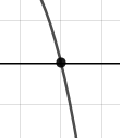
\includegraphics[width = 0.3\textwidth]{../Figures/polyZeroBehaviorCopyAC.png}\item 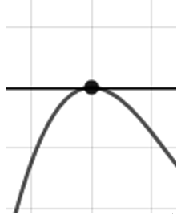
\includegraphics[width = 0.3\textwidth]{../Figures/polyZeroBehaviorCopyBC.png}\item 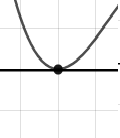
\includegraphics[width = 0.3\textwidth]{../Figures/polyZeroBehaviorCopyCC.png}\item 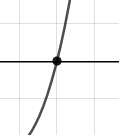
\includegraphics[width = 0.3\textwidth]{../Figures/polyZeroBehaviorCopyDC.png}\end{multicols}\item None of the above.
\end{enumerate} }
\litem{
Describe the end behavior of the polynomial below.\[ f(x) = 8(x - 4)^{5}(x + 4)^{8}(x + 5)^{2}(x - 5)^{4} \]\begin{enumerate}[label=\Alph*.]
\begin{multicols}{2}\item 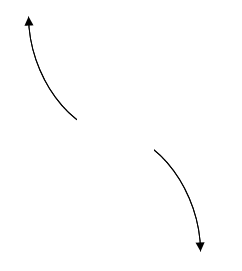
\includegraphics[width = 0.3\textwidth]{../Figures/polyEndBehaviorCopyAC.png}\item 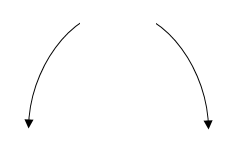
\includegraphics[width = 0.3\textwidth]{../Figures/polyEndBehaviorCopyBC.png}\item 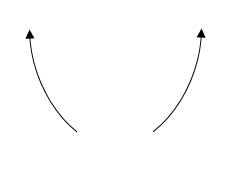
\includegraphics[width = 0.3\textwidth]{../Figures/polyEndBehaviorCopyCC.png}\item 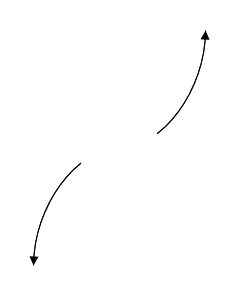
\includegraphics[width = 0.3\textwidth]{../Figures/polyEndBehaviorCopyDC.png}\end{multicols}\item None of the above.
\end{enumerate} }
\litem{
Which of the following equations \textit{could} be of the graph presented below?
\begin{center}
    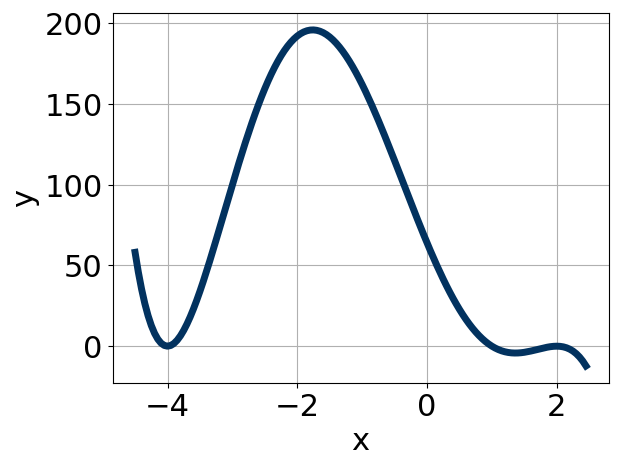
\includegraphics[width=0.5\textwidth]{../Figures/polyGraphToFunctionC.png}
\end{center}
\begin{enumerate}[label=\Alph*.]
\item \( -16(x - 2)^{8} (x - 3)^{5} (x + 2)^{7} \)
\item \( -2(x - 2)^{7} (x - 3)^{9} (x + 2)^{7} \)
\item \( 2(x - 2)^{10} (x - 3)^{8} (x + 2)^{9} \)
\item \( 6(x - 2)^{4} (x - 3)^{5} (x + 2)^{9} \)
\item \( 3(x - 2)^{11} (x - 3)^{5} (x + 2)^{11} \)

\end{enumerate} }
\litem{
Describe the zero behavior of the zero $x = 7$ of the polynomial below.\[ f(x) = -5(x + 7)^{9}(x - 7)^{14}(x - 9)^{5}(x + 9)^{6} \]\begin{enumerate}[label=\Alph*.]
\begin{multicols}{2}\item 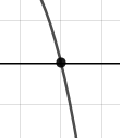
\includegraphics[width = 0.3\textwidth]{../Figures/polyZeroBehaviorAC.png}\item 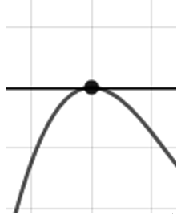
\includegraphics[width = 0.3\textwidth]{../Figures/polyZeroBehaviorBC.png}\item 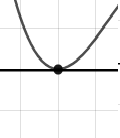
\includegraphics[width = 0.3\textwidth]{../Figures/polyZeroBehaviorCC.png}\item 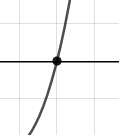
\includegraphics[width = 0.3\textwidth]{../Figures/polyZeroBehaviorDC.png}\end{multicols}\item None of the above.
\end{enumerate} }
\end{enumerate}

\end{document}